\section{Style model}
\label{sec:styles}
Several expressibility parameters exist to characterise motion. 
We used some of these parameters to filter pre-designed motions and to generate \textit{styled} motion.

Our definition of \emph{Behavioural Styles} is in line with psychological role-dependent styles, and hence takes into account the role played by the robot.
Before giving details in the model and the generation process of \textit{styled} behaviour, let us clarify the properties of our behavioural styles:
\begin{itemize}[noitemsep,nolistsep]
	\item[$\bullet$]  described by a list of parameters
	\item[$\bullet$]  expressed in non-verbal cues of communication
	\item[$\bullet$]  associated to a meaningful concept in psychology in order to be understandable by the end-user
	\item[$\bullet$]  associated to a role
\end{itemize}


\subsection{Design Approach}
In this section, the different modules involved in the style model are described. 
Then, we detail on the implementation and give some examples of style sheet and application on the Nao\footnote{Nao is a humanoid robot developed by Aldebaran}  and Reeti\footnote{Reeti is a PC-bot with doted with facial expression capabilities developed by Robopec} robots are given.


Styles characterise the plasticity of the behaviour (variability in the same context) as opposed to the personality that characterises the behaviour consistency (consistency across contexts).
On top of the roles, behavioural styles will affect the non-verbal expressibility within the role.

The notion of style is in this model: a set of behavioural changes that can be applied to any motion of a role repertoire and that leads to a meaningful interpretation of the way the motion is executed. 
A style filter is used to generate behaviours according to the role and to some preferences. 
Only a few styles have been implemented for our experiments but the solution that we propose can be extended.
The aim is that users could choose the styles from a catalogue and set the one they prefer, providing hence the adaptability of the companion within the social role. 

As for CSS, the objective in the style framework for design of social behaviour for robots is to make them \textbf{reusable }and \textbf{flexible}.
We intent then to show that styles can be applied to various gestures and pre-defined behaviour but also used for various robotic platforms. 


The style model acts similarly to a filter. 
It is fed by neutral gestures that are contained in the role repertoire and applied at run-time on the pre-selected gesture. 
The stylized gesture is then sent to the scheduler in order to perform it.


\begin{figure}[h]
	\centering
	\begin{tikzpicture}[node distance=2cm]
	\node (motion) [io2] {\scriptsize Role's Motion repertoire};
	\node (style) [io2, below of=motion] {\scriptsize BSS};
	\node (filter) [io2, right of=style] {\scriptsize Style filter};
	\node (postpross) [io2, right of=filter] {\scriptsize Post-Processing};
	\node (limits) [io2, above of =postpross] { \scriptsize Platform limits};
	\node (smotion) [io, right of=postpross] {\scriptsize Styled Motion};
	\draw [arrow] (style) -- (filter);
	%	\draw [arrow] (context) -- (filter);
	\draw [arrow] (motion) -- (filter);
	\draw [arrow] (filter) -- (postpross);
	\draw [arrow] (limits) -- (postpross);
	\draw [arrow] (postpross) -- (smotion);
	\end{tikzpicture}
	\caption{Pipeline of Stylistic treatment of data}
	\label{fig:workflowstyle}
\end{figure}

The figure \ref{fig:workflowstyle} shows the general data work-flow for the runtime generation of stylistic motion.
Our system takes as input a pre-defined motion that has been selected to be performed. 
This motion belongs to a motion repertoire that is associated to the current role played by the robot.
The input \textbf{motion} is defined by a series of key-frames.
A motion is hence a tuple containing : 
the names of the joints active during this motion,
for each joint the list of relative \textit{time} when a key-frames appends and for each joint and each time the associated \textit{key-frame} value (either angular or relative activation of the joint).

The styles are defined within the \textbf{Behavioural Style Sheet} (BSS) format. 
The style is set before run-time. 
It defines the modification that will be applied to the original motion.
The BSS is divided in two main parts, according to the previously mentioned situational inter-relation, the hearer and the speaker parts.
Indeed,  according to the fact that the robot is reacting to someone speaking or speaking itself, the style parameters may vary.
The BSS is further discussed in the section \ref{ssec:bss}.

The \textbf{Style filter} is the core program. 
Written in Python, it contains some transformation algorithms inspired from works in 3D animation allowing the interpretation of the BSS and the generation of new motion.
The generated motion can be however out-passing the physical constraints of the robot's motor. 

The \textbf{Post-Processing} module takes as input the platform's limits (speed and angular limits of each joints) and the generated motion and ensures that the computed styled motion is within these limits.
If not, the generated motion is modified to fit within the joints' constraints


\subsection{Style filter}
\label{ssec:bss}
We defined behavioural styles according to the 1) static and 2) dynamic parameters, as well as 3) decorators patterns. 
These parameters allow us to depict variation of execution of motions.
The values taken by these parameters are referred to psychological models of style and are used as a percentage of the total value in order to be applicable to several platforms or the frequency rate.
\begin{figure}
	\centering
	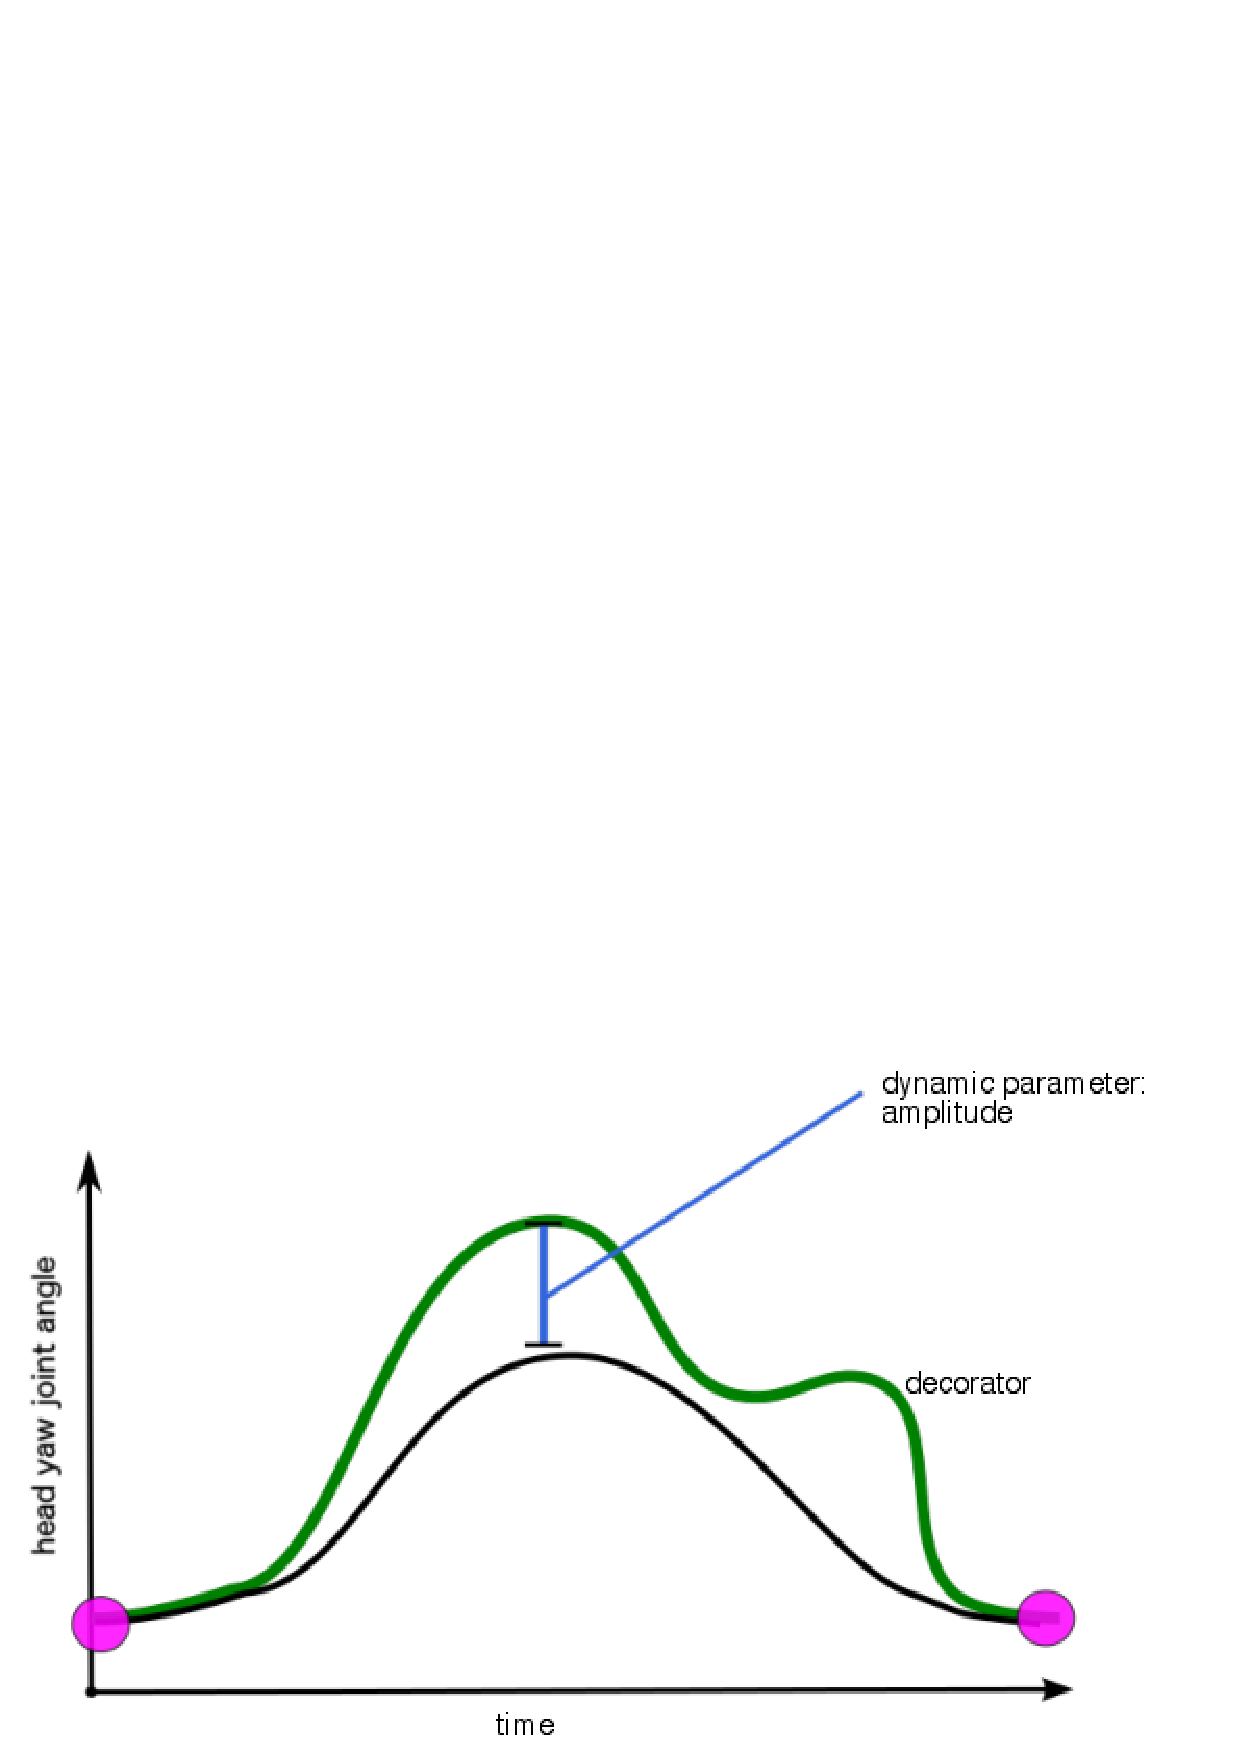
\includegraphics[width=0.8\linewidth]{Figures/illustrate/style_graph}
	\caption{Style parameters for Head Yaw(green is stylized motion, black is original, the P0 pose is in pink)}
	\label{fig:styles_parameters}
\end{figure}
%todo show more than 1 style and show noise
Figure \ref{fig:styles_parameters} shows an example of stylisation of a head yaw joint angle motion.
In this example, the static parameters are included in the $p0$ position.
The amplitude change is a part of the dynamic parameter. 
Finally the decorator is an additional keyframe with a new value. 
The decorator is often an additional motion that is fused with the current motion.

\paragraph{Static parameters} allow to describe the neutral pose \texttt{p0}. 
This neutral pose \texttt{p0} is the posture the robot will take by default.
Sometimes, some joints of the body won't be in motion,  and hence the robot will keep the joint values of \texttt{p0}.
As before, we define this pose in accordance with the styles found in the literature. 
There are several static parameters that exist to describe poses. 
\texttt{p0} is very platform dependent. 

The definition of the pose is made in a specific file for each robotic platform. 
The style modeller makes a reference to this file in order to build the stylized motion at runtime and adds p0 before and after each motion event to ensure that it is the default pose.




\paragraph{Dynamic parameters}
From the literature in HRI and virtual agents in the domains of animation and psychology, we have listed some dynamic parameters that can be useful to depict changes in styled motion.
The current implementation of styles take into account the following parameters. 
%todo put a bit more detail in how it works
\begin{itemize}[noitemsep,nolistsep]
	\item Amplitude: the spacial extent related to the dimension of expansiveness from Gallaher and Meharbian.
	\item Speed: temporal extent and the velocity of execution of the movement.
	\item Tempo: specifies a rhythm for the key-frames in the motion (that are spaced according to the tempo).
	\item Noise: opposed to fluidity, noise makes the movements jerky where smoothing makes the movement fluid.
\end{itemize}
These parameters are set for each style, and for each of them, an algorithm takes the current motion and the value of this dynamic parameter to compute a new motion.
For instance, one can double the amplitude, change the tempo to 10Hz, add noise to the motion or slow down the motion.

\section{Model Validation}
Prior to this experiment, a first online study was performed \cite{Johal2014}. 
This online study aimed to ensure that generated styles were perceptible by end-users. 
93 parents watched videos of robots with one of the two parenting styles, Permissive or Authoritative. 
This study showed that styles where expressible by both humanoid and facial expressive robots. 
We also found that preferred styles by parents did not match their own styles, which confirmed the fact that styles should stay a user controlled variable. 

After the on-line study, this experiment aimed to do a real user experiment in an ecological environment in order to test the credibility and the acceptability of styles by children. 